\part{Architecture}
\label{sec:Architeture}

In this part, the high-level structure of \LibName{} is defined. This is done in two refinement levels:
\begin{itemize}
\item The technical architecture shows the technical environment and parts of \LibName{}
\item The functional architecture shows and describes the functional components of \LibName{}
\end{itemize}

%===============================================================================================
%		General Design Decisions
%===============================================================================================

\chapter{General Design Decisions}
\label{sec:GeneralDesignDecisions}

This chapter presents all general design decisions that have a big impact on the overall architecture. It is usually very hard to revert any of those design decisions. As they generally affect the whole library, they have no direct relation to specific requirements, but build the framework to be able to fullfill those requirements.

%-----------------------------------------------------------------------------------------------
%		Design Decision: \JavaVersion
%-----------------------------------------------------------------------------------------------

\section{Using \JavaVersion{}}
\label{sec:VerwendungVonJava}

\DD{dd:001}
{% Title
\LibName{} is based on \JavaVersion{}%
}
{% Short description
\LibName{} is developed based on the ``latest update'' of \JavaVersion{}. Migrating \LibName{} towards newer Java versions is considered on a regular basis.
}
{% Rationale
Java as programming language is well established and in wide use by a big number of world-wide developers. Furthermore, Java is platform-independent. In principle, porting \LibName{} to other platforms, to Java ME or to Java for  e.g. smart phones (e.g. Android) should be less effort than porting an equivalent C/C++ library. The author has long experience with Java programming, so this should facilitate productivity. The competitor libraries in the Java environment are good, but \LibName{} can be even better. The current (state 28th of November 2017) version \JavaVersion{} is used, because we want to create a modern library using the newest language features, libraries and programming models in the Java world. Furthermore, it is guaranteed that we get longer support for this Java version than for the previous ones.
}
{% Disadvantages
Applications being based on Java 7, Java 8 or older are not supported by \LibName{}. This would especially effect Java EE applications where it seems not yet possible to use \JavaVersion{} for some application servers.
}

%-----------------------------------------------------------------------------------------------
%		Design Decision: Use of 3rd Party Libraries
%-----------------------------------------------------------------------------------------------

\section{Use of 3rd Party Libraries}
\label{sec:VerwendungAndLib}

\DD{dd:002}
{% Title
\LibName{} uses as few 3rd party libraries as possible
}
{% Short description
\LibName{} uses mostly only the libraries offered by Java SE. In the productive code of the library, no dependencies to other 3rd party libraries are used except for logging.
}
{% Rationale
Additional dependencies could create overhead or question marks when it comes to building, shipping, testing or licensing. Furthermore, you might at one point in time reuse a well-tested and documented 3rd party library, and in the next year, it might get abandoned or bugs show up that do not get fixed. We ensure that bugs are just bugs that we can fix ourselves and we do not depend on other library developers.
}
{% Disadvantages
Sometimes this might mean ``do it yourself'' instead of reuse.
}

%-----------------------------------------------------------------------------------------------
%		Design Decision: Component-based Library
%-----------------------------------------------------------------------------------------------

\section{Component-based Library}
\label{sec:KomponentenbasierteLibrary}

\DD{dd:003}
{% Title
\LibName{} is component-based
}
{% Short description
\LibName{} is consisting of so-called components as defined in the follow-up sub-section. Each component has a well defined responsibility, a public API that can be used by all other components as well as a private implementation part that must not be used by other components. 
}
{% Rationale
Structuring a big library into modular parts helps to manage the complexity of the library during planning, design, implementation and maintenance. By using a reasonable component structure, clear responsibilities, dependencies and decoupling of unrelated parts is achievable. Changes in implementation parts of a component do have less probability to affect other components, as they do only depend on the API of the component.
}
{% Disadvantages
Probably a little bit more overhead due to sometimes following ``conventions'' where an easier structure would be possible
}

%-----------------------------------------------------------------------------------------------

\subsection{Definition of the component term}
\label{sec:ComponentTermDefinition}

A \emph{component} in \LibName{} is \emph{a self-contained software module with clearly defined task}. It offers \emph{services} the can be used via a \emph{well-defined interface (API)}. These services are used both by the users of \LibName{} as well as by other components of the library. 

The following figure shows a component in \LibName{} schematically:

\begin{figure}[H]
\centering
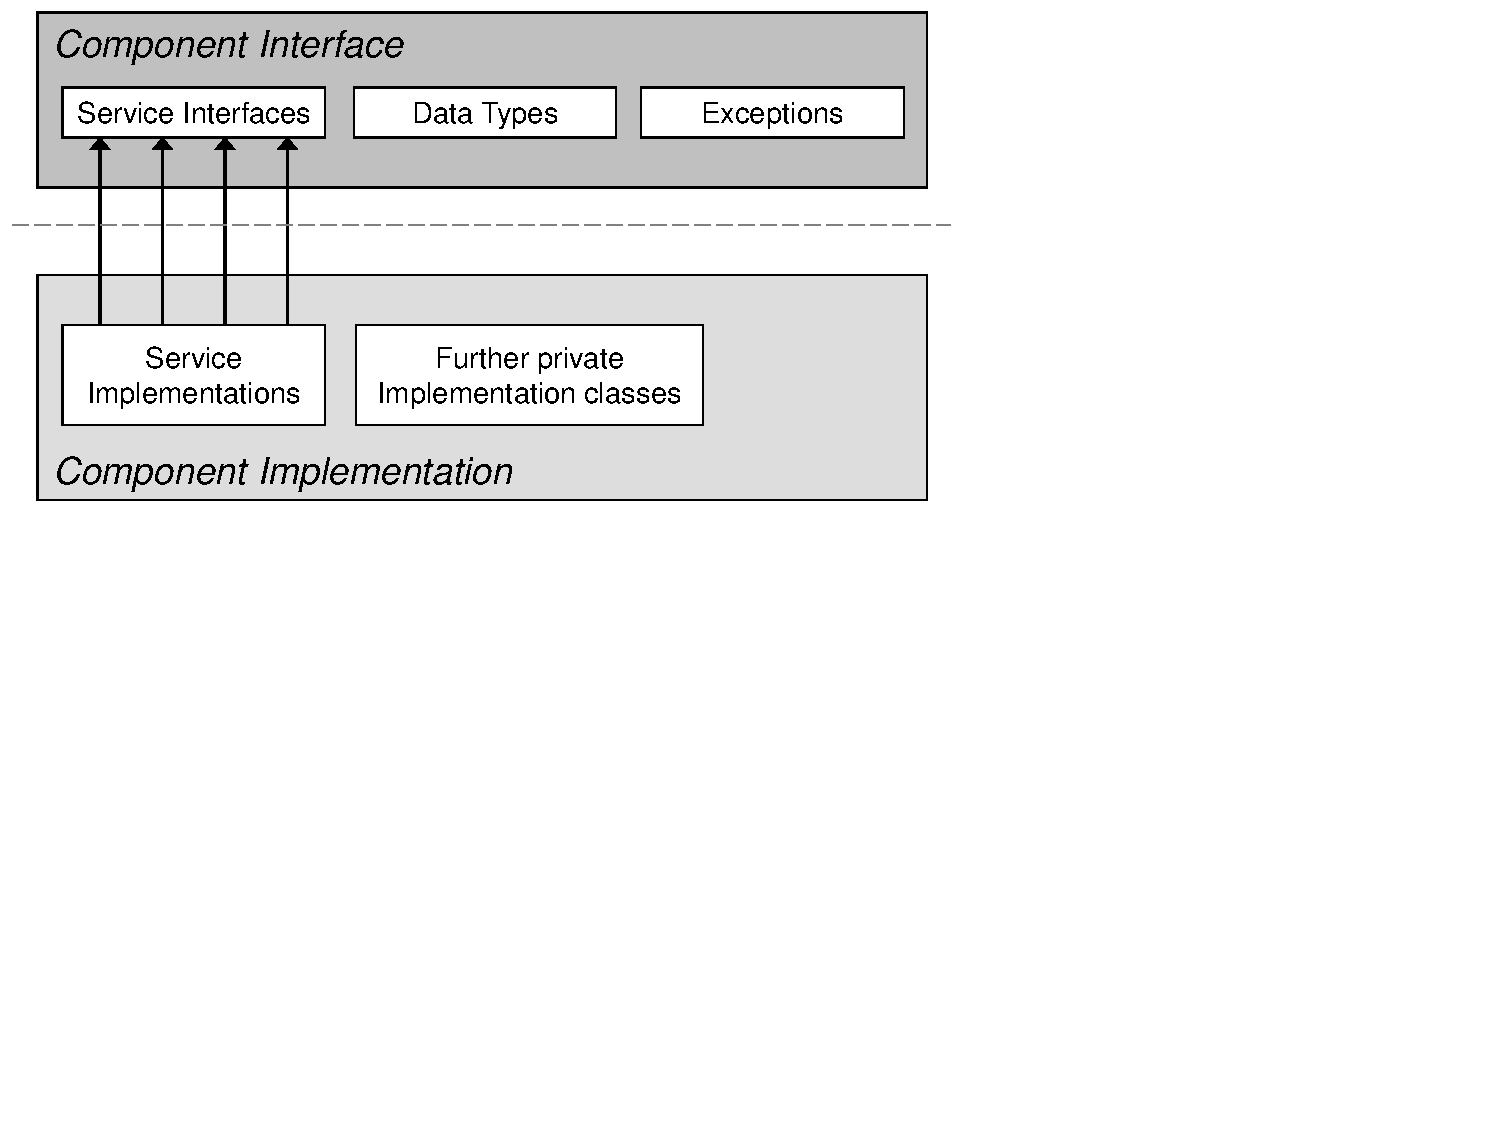
\includegraphics[width=1.00\textwidth]{figures/II_ComponentStructure.pdf}
\caption{Structure of a component}
\label{fig:5_3_SCH_Komponente}
\end{figure}

A component interface consists of one or more Java interfaces, the so-called service interfaces, exceptions as well as data types.
\begin{itemize}
\item \emph{Service interfaces} offer the functional API of the component, each method corresponds to a service of the component. A single Java interface is use for a clear defined subtask of the component. Some service interface have factory methods that provide access to further service interfaces of the component.
\item \emph{Data types} are (mostly) constant Java classes that are usually used to hold data for service input and output parameters. Usually they are value types, but sometimes they are also representing a specific entity such as a medium.
\item \emph{Exceptions} are functional errors. These are mostly unchecked exceptions signaling a specific error condition, in rare cases we use unchecked exceptions if the caller can handle the situation.
\end{itemize}

In addition, a component might have data ownership for a specific kind of relevant data. This means that this data can only be read or manipulated via using the public API of this component, and by no other means.

%-----------------------------------------------------------------------------------------------

\subsection{Design Decision for using components}
\label{sec:DesVerwKomp}

%-----------------------------------------------------------------------------------------------
%		Design Decision: Components decoupled by a light-weight service locator pattern
%-----------------------------------------------------------------------------------------------
\DD{dd:004}
{% Title
Components decoupled by a light-weight service locator pattern
}
{% Short description
To ensure low coupling between components, they must know each other only via their interfaces. A component can obtain a reference to a service implementation without directly depending on the implementation class itself by using a service locator pattern, specifically the Java SE \texttt{ServiceLoader}.
}
{% Rationale
We want to decouple components. To achieve this, it must not be allowed for components to instantiate service implentations of other components directly, because service implementations are not part of the public interface of a component. A service locator exactly offers to obtain a service implementation reference without depending on it. For a library such as \LibName{}, neither JavaEE nor Spring or CDI dependency injection are valid options. Google Guice is not chosen because of \DesLink{dd:002}. Java SE \texttt{ServiceLoader} is a very easy to use and fully sufficient facility.
}
{% Disadvantages
No disadvantages known
}

%-----------------------------------------------------------------------------------------------
%		Design Decision: Singleton Components
%-----------------------------------------------------------------------------------------------

\DD{dd:005}
{% Title
Singleton Components
}
{% Short description
Each component offers a single \emph{main API service interface} that itself offers access to any other service interface the component provides.

From a runtime perspective, each main API service interface thus has a single (ideally stateless) implementation, which you could refer to as ``singleton''.
}
{% Rationale
A main API service interfaces is purely procedural. There is just one implementation of component allowed at runtime. We just need one instance for each component at runtime, as it is stateless. This safes memory and initialization overhead.
}
{% Disadvantages
No disadvantages known
}

%-----------------------------------------------------------------------------------------------
%		Design Decision: API and Implementation Layers
%-----------------------------------------------------------------------------------------------

\DD{dd:007}
{% Title
API and Implementation Layers
}
{% Short description
Each component offers its services, exceptions and data types on an \emph{API layer}. This layer is a horizontal layer cutting through the whole library and representing the public API of the library. Also per component, it is the public API of a component. Compile-time dependencies from user code to \LibName{} as well as between components are only allowed via this API layer. The implementation layer depends on the API layer and contains any private classes. An outside component and user code is not allowed to have a compile-time dependency to implementation layer classes
}
{% Rationale
Clear separation of concerns and information hiding. What implementation layer classes do is their private business, nobody from the outside world is allowed to directly work with and depend on them.
}
{% Disadvantages
No disadvantages known
}

%-----------------------------------------------------------------------------------------------
%		Design Decision: No further subdivision of implementation layers
%-----------------------------------------------------------------------------------------------

\DD{dd:008}
{% Title
No further subdivision of implementation layer
}
{% Short description
It is not necessary to further subdivide the implementation layer into sublayers. Instead, each component can have an arbitrary package structure in its implementation layer code.
}
{% Rationale
We do not see any reasonable sublayers for \LibName{} that could be relevant for all components of the library.
}
{% Disadvantages
No disadvantages known
}

%-----------------------------------------------------------------------------------------------
%		Design Decision: Development Environment
%-----------------------------------------------------------------------------------------------

\section{Development Environment}
\label{sec:entw}

\DD{dd:009}
{% Title
Development Environment
}
{% Short description
As development environment, we use Maven, Eclipse and SubVersion for \LibName{}.
}
{% Rationale
Amazing toolset that leaves not much else to wish for.
}
{% Disadvantages
No disadvantages known
}

%-----------------------------------------------------------------------------------------------
%		Design Decision: Multithreading
%-----------------------------------------------------------------------------------------------

\section{Multithreading}
\label{sec:mult}

\DD{dd:010}
{% Title
\LibName{} is not thread-safe
}
{% Short description
\LibName{} is not a thread-safe library and (usually) does not use any Java APIs that are thread-safe.
}
{% Rationale
In some cases, thread-safety means performance degradation due to synchronisation points. In addition, it almost always means higher complexity. In a non-functional programming language such as Java with a lot of mutable state, it is hard to get thread-safety right. If users need to work with \LibName{} in multiple threads, they have to ensure thread-safety themselves.
}
{% Disadvantages
No disadvantages known
}

%-----------------------------------------------------------------------------------------------
%		Design Decision: Architecture
%-----------------------------------------------------------------------------------------------

\section{Architecture}
\label{sec:arch}

\DD{dd:011}
{% Title
Architecture of \LibName{}
}
{% Short description
\LibName{}'s architecture adheres to the technical and functional architecture as descrived in chapters \SectionLink{sec:TechnicalArchitectureChap} and \SectionLink{sec:FunctionalArchitectureChap}.
}
{% Rationale
See architecture discussion in detail in the next chapters
}
{% Disadvantages
See architecture discussion in detail in the next chapters
}

%===============================================================================================
%		Technische Archiktur
%===============================================================================================

\chapter{Technical Architecture}
\label{sec:TechnicalArchitectureChap}

The technical architecture allows functional components (i.e. components offering the actual functionality of \LibName{}) to operate in their technical infrastructure. In addition, the technical architecture consists of the layers of each component. We have a component-based layered architecture as defined in \SectionLink{sec:KomponentenbasierteLibrary}. The layering has already been defined in the design decisions \DesLink{dd:007} and \DesLink{dd:008}. Thus, we just concentrate on a brief overview of the technical infrastructure and the technical base components here.

%-----------------------------------------------------------------------------------------------
%		Technische Infrastruktur
%-----------------------------------------------------------------------------------------------

\section{Technical Infrastructure}
\label{sec:TechnicalInfrastructure}

The technical infrastructure describes the environment required to work with \LibName{} as shown in the following figure:

\begin{figure}[H]
\centering
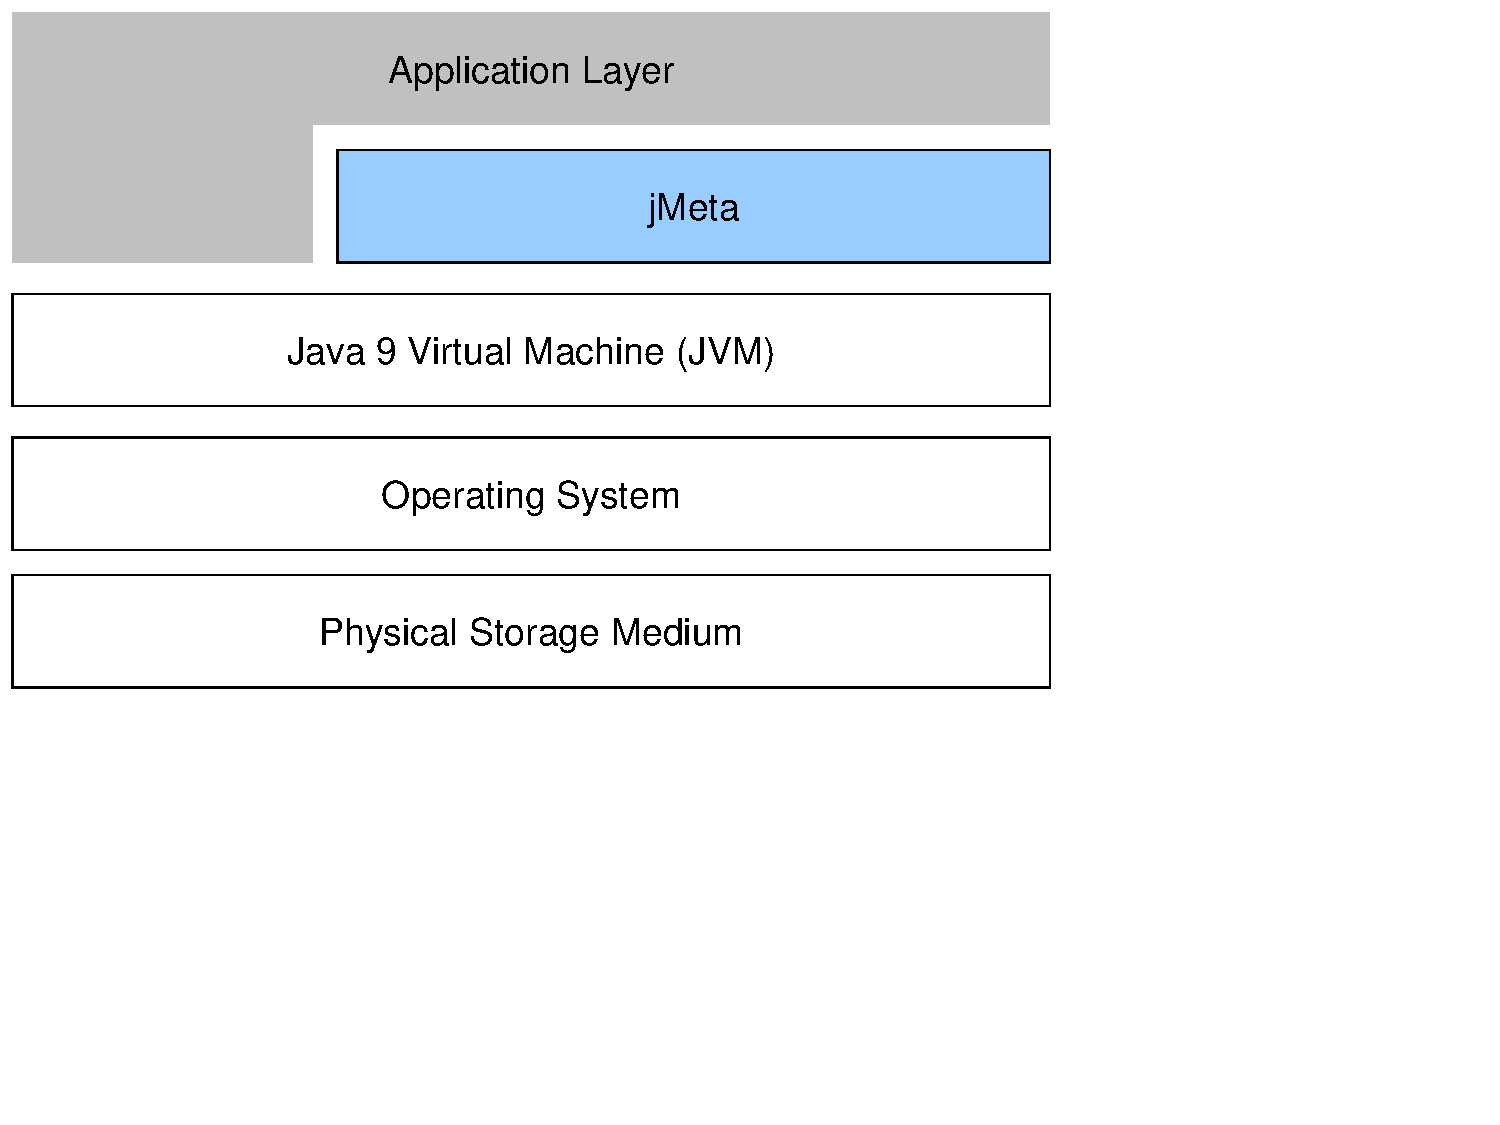
\includegraphics[width=1.00\textwidth]{figures/II_TechnicalInfrastructure.pdf}
\caption{Technical infrastructure of \LibName{}}
\label{fig:5_3_SCH_TechnicalInfrastructure}
\end{figure}

The technical layers can be interpreted as dependency and communication structure. The application layer is based on \LibName{}, while \LibName{} as well as the application layer uses \JavaVersion{}. Thanks to this, the library and its using applications are platform-independent and can be used on any platform currently supported by Java. \JavaVersion{} accesses the operating system, which offers services to access the physical medium.

However, \LibName{} is only developed for \JavaVersion{} and cannot be used by applications requiring earlier versions.

Each layer only accesses the neighouring layer.

%-----------------------------------------------------------------------------------------------
%		Technical Base Components
%-----------------------------------------------------------------------------------------------

\section{Technical Base Components}
\label{sec:TechnicalBasis}

Technical base components are just helpers providing a framework and basis for the functional components of \LibName{}. With ``functional'' we are referring to the tasks of the library, i.e. reading and writing metadata and reading container data. The necessary base components are:
\begin{itemize}
\item Logging
\item Service-Locator to achieve a component oriented architecture
\item Utility
\item Maintaining extensions
\end{itemize}

Details of these components are given in \SectionLink{sec:Design}.

%===============================================================================================
%		Functional Architecture
%===============================================================================================

\chapter{Functional Architecture}
\label{sec:FunctionalArchitectureChap}

The functional Architecture defines the structuring of the library into functional units, so called functional components according to \SectionLink{sec:KomponentenbasierteLibrary}. For completeness, also the dependencies of the functional components with the technical base components is shown in functional architecture diagrams. In addition, the functional architecture also contains basic functional design decisions influencing the direction of the whole library.

%-----------------------------------------------------------------------------------------------
%		Fundamental design decisions of \LibName{} functionality
%-----------------------------------------------------------------------------------------------

\section{Fundamental design decisions of \LibName{} functionality}
\label{sec:Grld}

The following design decisions are fundamental for the whole library and mostly have a cross-cutting effect. They form the basis for the functional design of all functional library components.

%-----------------------------------------------------------------------------------------------

\DD{dd:101}
{% Title
Generic reading and writing according to a format specification
}
{% Short description
Reading and writing different \TERMcontainerFormat{}s is done generically by a central component. A format specification describes which features a \TERMcontainerFormat{} has, especially how its \TERMdataBlock{}s are structured and how they need to be interpreted. Thus it can be seen as a kind of generic parsing (and writing and validating) instruction of the data format.
}
{% Rationale
According to the document \cite{MC17}, \TERMcontainerFormat{}s and their more specific children \TERMmetadataFormat{}s have a lot of things in common, in specific the way how they are structured and parsed. These common properties can be descrubed using a generic format specification. Instead of rewriting specific parsing, writing and validation code for each new supported \TERMcontainerFormat{}, all of them can be implemented by the same generic parsing, writing and validation code that is based on the generic format specification.

This way, in the end, there should be less code, less duplication, and also a higher quality of code as it can be tested easier.

This design decision also essentially enables to meet the requirement \SectionLink{sec:REQ007ErweiterbarkeitUmNeueMetadatenUndContainerformate}, as this way it is much easier to extend the library with new \TERMcontainerFormat{}s.
}
{% Disadvantages
The generic code can probably not be written to support any and every possible future or existing \TERMcontainerFormat{} out of the box. Thus there might still be changes required in future. We have to carefully avoid to add format specific code to this generic core code, such that it not again becomes a complex monster, where in the end it would have been better to rewrite code for each extension. The latter risk exists if the formats do not have as much in common as assumed by this design decision. This can make testing or even understanding the generic code extensively hard.

In addition, there might be some small performance drawbacks, as generic code can of course not as heavily and specifically tuned as format-specific code can.
}

To mitigate the possible disadvantages of \DesLink{dd:101}, we define the following design decision:

%-----------------------------------------------------------------------------------------------

\DD{dd:102}
{% Title
It is possible to override generic reading and writing in extensions
}
{% Short description
\LibName{} \TERMcontainerFormat{} extensions are allowed to override specific parts of reading, writing and validation code to adapt them to specifics of their data format.
}
{% Rationale
This minimizes the disadvantages of \DesLink{dd:101}. In special cases, this can lead to easier or faster implementations. Furthermore, using such hooks, it might not be necessary to blow up the core code by specifics that are actually only relevant for one or just a few concrete formats. Those specifics can then be implemented in the corresponding format's code.
}
{% Disadvantages
It might not be easy to clearly define and communicate which parts can be overridden and which not.
}

To also mitigate the risk of too big and complex generic core code, we define:

%-----------------------------------------------------------------------------------------------

\DD{dd:103}
{% Title
Format specifics are only defined in extensions
}
{% Short description
Any special features of a \TERMcontainerFormat{} or \TERMmetadataFormat{} that are no common properties/features of a lot of container formats are only defined in the corresponding extensions. That said, the generic core code never directly depends on specifics of data formats, neither syntactically (e.g. compile-time dependencs to format extension; by using if-then-else to do things different depending on the current format) or semantically (e.g. implementing a special feature for just one format, but claim it is ``generic''). Only if a special feature of a format can be brought down to a common denominator for all supported formats, it is implemented generically.
}
{% Rationale
There is a strict separation between core implementation and format specifics, which allows better handling of the overall complexity.
}
{% Disadvantages
No disadvantages known
}

%-----------------------------------------------------------------------------------------------

\DD{dd:100}
{% Title
High-level and low-level API
}
{% Short description
The generic, format-independent core parts of \LibName{} form a kind of \emph{low-level API} for parsing, writing and validating data of a \TERMcontainerFormat{} quite generically down to the byte level. The end user of \LibName{} is allowed to use this part of the library directly.

However, on top of that there is a more convenient and format-specific \emph{high-level API} the user usually uses to access data.
}
{% Rationale
According to \DesLink{dd:101}, \LibName{} has a generic format-independent core part. This could be made private, not to be used by end users of \LibName{}. However, this would not make it possible to fullfill \SectionLink{sec:REQ004ZugriffAufAlleRohdatenUeberDieLibrary}. At the same time, format-specific extensions need to reuse the core part. We do not want to throw the core part together with these higher-level extensions.
}
{% Disadvantages
No disadvantages known
}

%-----------------------------------------------------------------------------------------------
%		Extensions
%-----------------------------------------------------------------------------------------------

\section{Extensions}
\label{sec:KompExt}

An \emph{extension} summarizes format-specific content for a given data format, or multiple variations of the data format. Per data format defined by the extension, these are (compare \DesLink{dd:101}, \DesLink{dd:102} and \DesLink{dd:103}):
\begin{itemize}
\item A data format specification which defines \TERMdataBlock{}s and their structure and relations.
\item An end-user high-level API to comfortably work with the data format, e.g. for creation of \TERMdataBlock{}s etc.; this API especially holds the data format identifier which the user can use to work with other components.
\item Implementation extensions that might override generic parsing, writing and validation.
\end{itemize}

As a ground rule, every single extension can but should not define extension code for more than one data format. It might expose more data formats only if these two data formats heavily overlap and are based on each other, e.g. ID3v1 and ID3v1.1. This is to fulfill the requirement \SectionLink{sec:REQ010SchreibenInAnderesAusgabemediumUnterstuetzt}.

Moreover, distinct extensions should never depend on each other, but only on the \LibName{} core to avoid any confusion for the user.

%-----------------------------------------------------------------------------------------------
%		Functional Architecture Components
%-----------------------------------------------------------------------------------------------

\section{Functional Architecture Components}
\label{sec:Subsystems}

The following component diagram shows the functional and technical base components of \LibName{} and their dependencies. An arrow indicates a necessary compile-time dependency. For each format extension, there is exactly one component.

\begin{figure}[H]
\centering
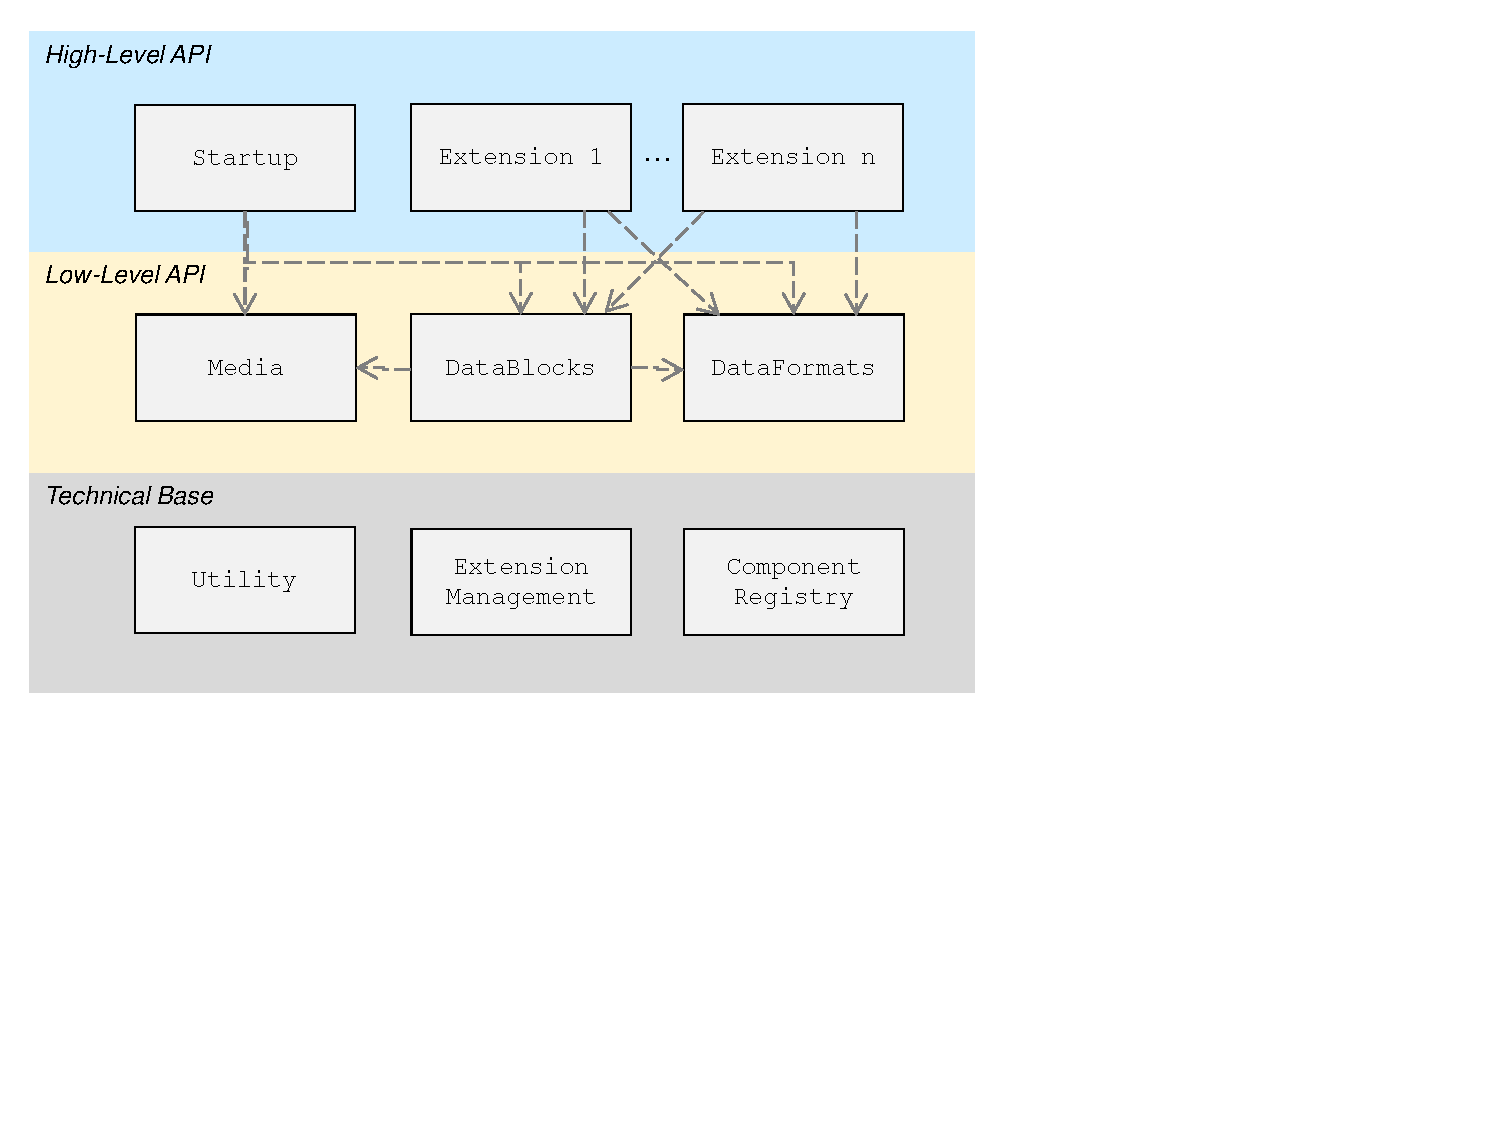
\includegraphics[width=1.00\textwidth]{figures/II_FunctionalArchitecture.pdf}
\caption{Component diagram of \LibName{}}
\label{fig:5_3_SCH_TechnicalArchitecture}
\end{figure}

You can identify a kind of ``component layering'' (not to be confused with the architecture layering, it is just a grouping of components). At the lowest level we have the technical base components, then followed up by the low-level API components and the high-level API (according to \DesLink{dd:100}) on top.

Dependencies to the technical base components are not shown in this diagram, as anybody can (and usually does) depend on them. Note that, due to this, we only list dependencies to technical base components in the component characteristics sections to follow if these dependencies are important and need to be specifically mentioned.

All the components displayed are just briefly described in the next sections.

%-----------------------------------------------------------------------------------------------
%		Component Characteristics
%-----------------------------------------------------------------------------------------------

\section{Component Characteristics}
\label{sec:StructureofaComponentDescription}

All components are briefly described by a common structure that looks like this:

\textbf{Component Name:} The name of the component.

\textbf{Task:} The main responsibility of the component.

\textbf{Controlled Data:} Any data the component has ownership for.

\textbf{Depends on $<$Component Name$>$:} Occurring multiple times, once for each component it depends on with a reason why this dependency is necessary.

%-----------------------------------------------------------------------------------------------

\section{Component \COMPcontext{}}
\label{sec:COMPContext}

\textbf{Component Name:} \COMPcontext{}

\textbf{Task:} The entry point for every user to \LibName{}. It loads all extensions and provides access to all other components of the library.

\textbf{Controlled Data:} Keine.

\textbf{Depends on \COMPextensionManagement{}:} \COMPcontext{} loads all extensions by using this component.

\textbf{Depends on \COMPcomponentRegistry{}:} \COMPcontext{} uses this component to instantiate all component singletons the user asks for.

%-----------------------------------------------------------------------------------------------

\section{Any extension component}
\label{sec:ExtComp}

\textbf{Component Name:} Arbitrary, usually the name of the data format the extension implements

\textbf{Task:} Offers the high-level API to work with the data format it implements.

\textbf{Controlled Data:} None.

\textbf{Depends on \COMPextensionManagement{}:} It needs this dependency to the extension framework because it is an extension.

\textbf{Depends on \COMPdataFormatManagement{}:} It implements a specific data format, does needs to depend on data format base classes defined in \COMPdataFormatManagement{}.

\textbf{Depends on \COMPdataPartManagement{}:} Extensions are allowed to override reading, writing and validation of data, thus they can depend on \COMPdataPartManagement{}.

%-----------------------------------------------------------------------------------------------

\section{Component \COMPdataPartManagement{}}
\label{sec:COMPdataPartManagement}

\textbf{Component Name:} \COMPdataPartManagement{}

\textbf{Task:} Implements generic reading and writing of \TERMcontainerFormat{}s and \TERMmetadataFormat{}s according to their format specification.

\textbf{Controlled Data:} Accessing raw \TERMcontainer{} or \TERMtag{} data on byte or bit level is only allowed by using this component.

\textbf{Depends on \COMPmedia{}:} \COMPdataPartManagement{} must read and write data portions from an external medium, for this it uses \COMPmedia{}.

\textbf{Depends on \COMPdataFormatManagement{}:} Needs access to the data format specification by depending on \COMPdataFormatManagement{}. This is necessary to implement the generic reading and writing.

%-----------------------------------------------------------------------------------------------

\section{Component \COMPdataFormatManagement{}}
\label{sec:COMPdataFormatManagement}

\textbf{Component Name:} \COMPdataFormatManagement{}

\textbf{Task:} Manages the generic data format definitions for \TERMcontainerFormat{}s.

\textbf{Controlled Data:} Has control over the data format specifications.

\textbf{Depends on:} No other components except technical base components.

%-----------------------------------------------------------------------------------------------

\section{Component \COMPmedia{}}
\label{sec:COMPmediumAccess}

\textbf{Component Name:} \COMPmedia{}

\textbf{Task:} Offers primitive to read and write all supported physical \TERMmedium{}. Hides medium access differences for other components.

\textbf{Controlled Data:} Accessing data of external media is only allowed by using \COMPmedia{}.

\textbf{Depends on:} No other components except technical base components.

%-----------------------------------------------------------------------------------------------

\section{Component \COMPextensionManagement{}}
\label{sec:COMPextensionManagement}

\textbf{Component Name:} \COMPextensionManagement{}

\textbf{Task:} Manages all extensions of \LibName{} generically, i.e. loading and verification.

\textbf{Controlled Data:} Descriptive data for extensions can only be obtained using \COMPextensionManagement{}.

\textbf{Depends on:} No other components except utility.

%-----------------------------------------------------------------------------------------------

\subsection{Component \COMPcomponentRegistry{}}
\label{sec:COMPcomponentRegistry}

\textbf{Component Name:} \COMPcomponentRegistry{}

\textbf{Task:} Implements the service locator functionality to enable components to depend only on the API of another component.

\textbf{Controlled Data:} Only via \COMPcomponentRegistry{}, access to metadata about components of \LibName{} is possible.

\textbf{Depends on:} No other components except utility.

%-----------------------------------------------------------------------------------------------

\subsection{Component \COMPutility{}}
\label{sec:COMPutility}

\textbf{Component Name:} \COMPutility{}.

\textbf{Task:} Offers diverse (technical) cross-functional stuff that needs to be used by most if not all other components, e.g. helper functionality to implement design-by-contract.

\textbf{Controlled Data:} None.

\textbf{Depends on:} No other components.

%###############################################################################################
%###############################################################################################
%
%		File end
%
%###############################################################################################
%###############################################################################################


%%% Local Variables:
%%% mode: latex
%%% TeX-master: "jMetaDesignConcept"
%%% End: